In this chapter we move away from the ScatterNet ideas from the previous 
chapters and instead look at using the wavelet domain as a new space in which to
learn. With ScatterNets, complex wavelets are used to scatter the energy into
different channels (corresponding to the different wavelet subbands), before the
complex modulus demodulates the signal to low frequencies. These channels can
then be mixed before scattering again (as we saw in the learnable scatternet),
but the progressive stages all result in a steady demodulation of signal energy
towards zero frequency. 

In this chapter we introduce the \emph{wavelet gain layer}
which starts in a similar fashion to the ScatterNet -- by taking the $\DTCWT$ of
a multi-channel input. Next, instead of taking a complex modulus, we learn a 
complex gain for each subband in each input channel. A single value here can 
amplify or attenuate all the energy in one part of the frequency plane. Then, 
while still in the wavelet domain, we mix the different input channels by subband (e.g.
all the $15\degs$ wavelet coefficients are mixed together, but the $15\degs$ and
$45\degs$ coefficients are not). We can then return to the pixel
domain with the inverse wavelet transform. 

We also briefly explore the possibility of doing nonlinearities in the wavelet
domain. The goal being to ultimately connect multiple wavelet gain layers
together with nonlinearities before returning to the pixel domain. 

The proposed wavelet gain layer can then be used in conjunction with regular
convolutional layers, with a network moving into the wavelet or pixel space and
learning filters in one that would be difficult to learn in the other.

Our experiments so far have shown some promise. We are able to learn complex
wavelet gains and a network with one or two gain layers shows small improvements.
However, with three or more such layers (in an 6 layer network) the network performance 
degrades. 

Additionally, we have not been successful in finding a nonlinearity that works
well in the wavelet domain. 

\section{Related Work}\label{sec:ch6:related} 
\subsection{Wavelets as a Front End}
Fujieda et.\ al.\ use a DWT in combination with a
CNN to do texture classification and image annotation 
\cite{fujieda_wavelet_2017, fujieda_wavelet_2018}. In particular, they take a
multiscale wavelet transform of the input image, combine the actviations at each
scale independently with learned weights, and feed these back into the network
where the activation resolution size matches the subband resolution. The
architecture block diagram is shown in \autoref{fig:ch6:fujieda}, taken from the
original paper.  This work found that their dubbed `Wavelet-CNN' could
outperform competetive non wavelet based CNNs on both texture classification and
image annotation.

\begin{figure}[bt]
  \centering
  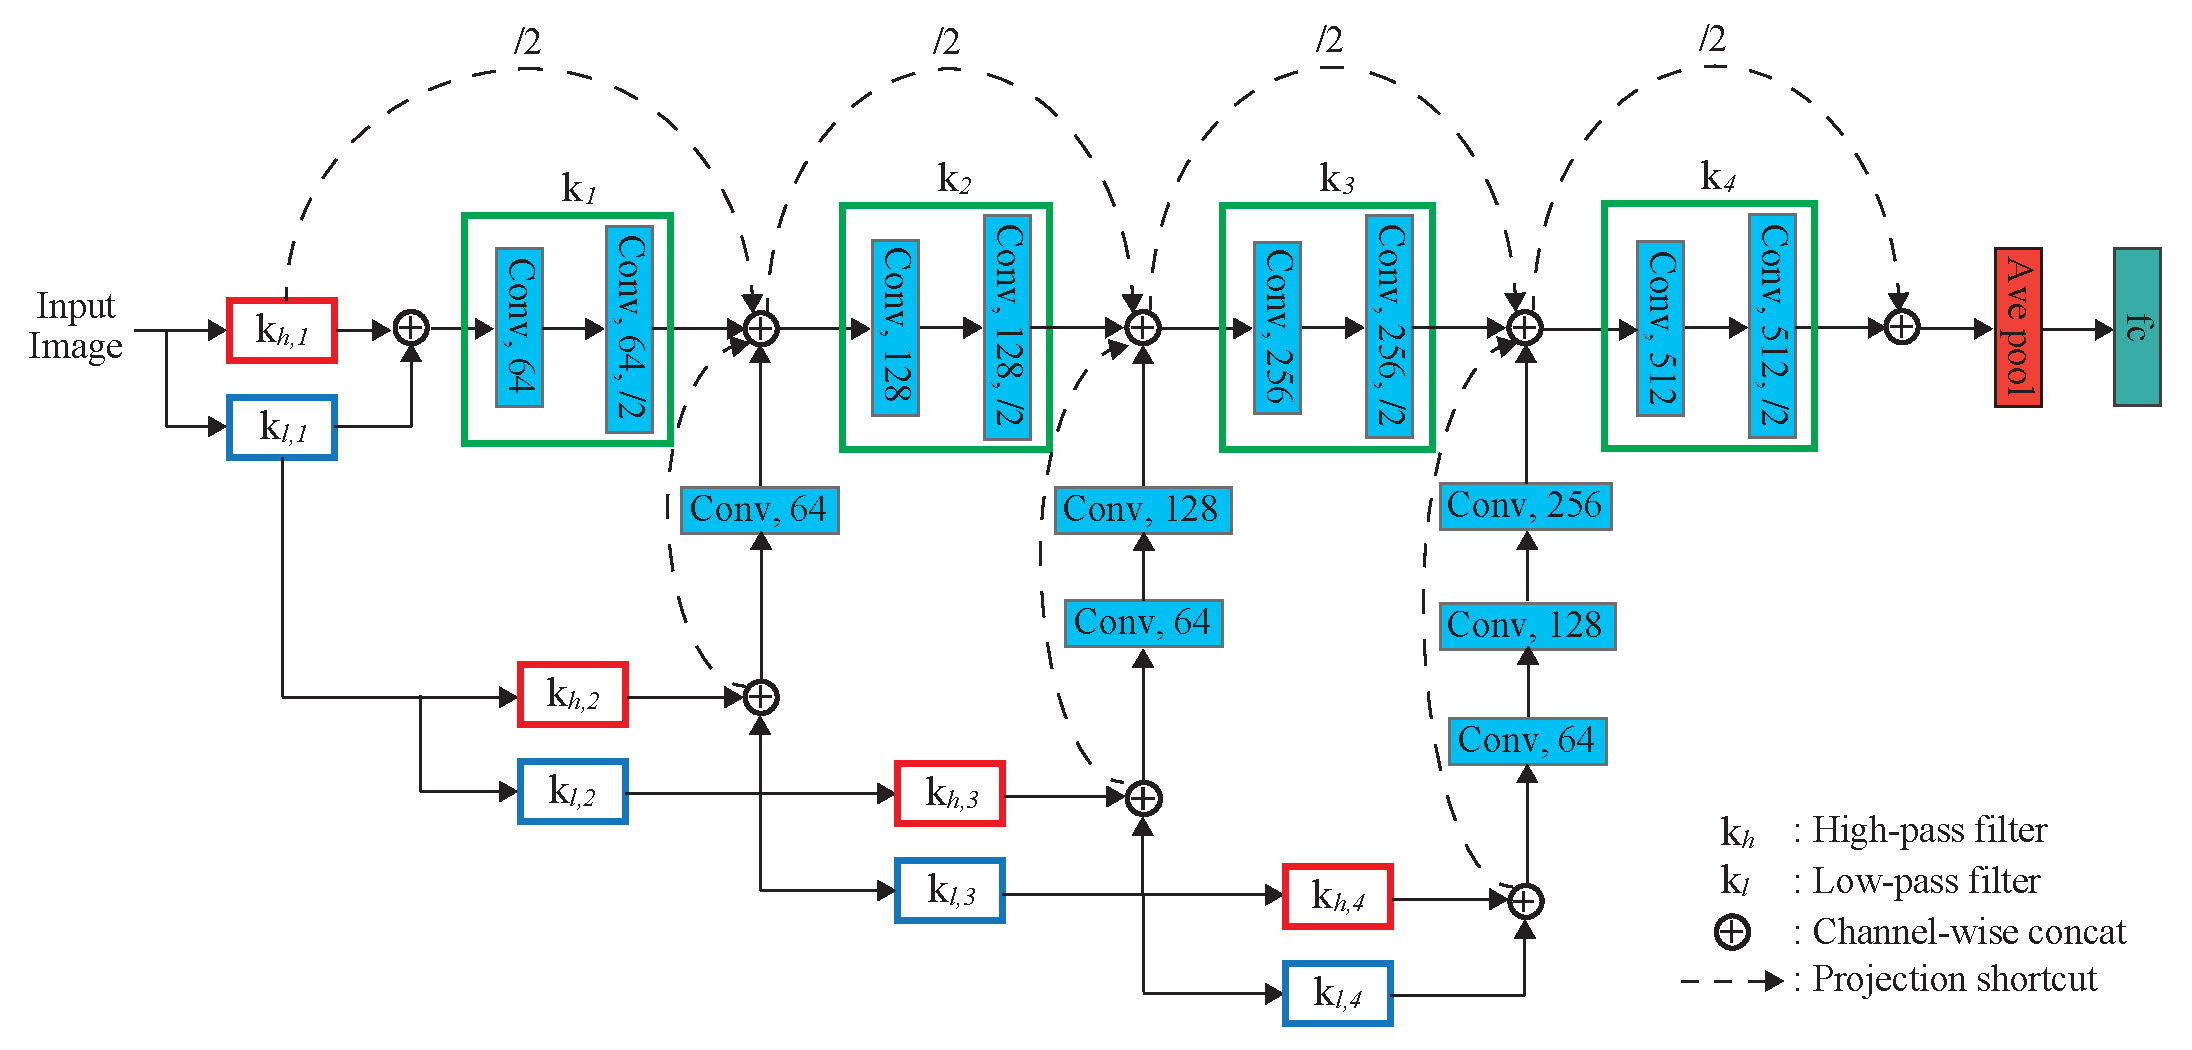
\includegraphics[width=\textwidth]{\imgpath/wavelet_CNN_3.pdf}
  \mycaption{Architecture using the DWT as a frontend to a CNN}{Figure 1 from
  \cite{fujieda_wavelet_2018}. Fujieda et.\ al.\ take a multiscale wavelet
  decomposition of the input before passing the input through a standard
  CNN\@. They learn convolutional layers independently on each subband and feed
  these back into the network at different depths, where the resolution of the
  subband and the network activations match.}
  \label{fig:ch6:fujieda}
\end{figure}

Several works also use wavelets in deep neural networks for super-resolution
\cite{guo_deep_2017} and for adding detail back into dense pixel-wise
segmentation tasks \cite{ma_detailed_2018}. These typically save wavelet
coefficients and use them for the reconstruction phase, so are a little less
applicable than the first work.


\section{Background and Notation}
We make use of the 2-D $Z$-transform to simplify our analysis:
%
\begin{equation}
  X(\zz) = \sum_{n_1}\sum_{n_2} x[n_1, n_2]z_1^{-n_1}z_2^{-n_2} =
  \sum_{\nn}x[c, \nn]\zz^{-\nn}
\end{equation}
%
As we are working with three dimensional arrays (two spatial and one channel) but are
only doing convolution in two, we introduce a slightly modified 2-D $Z$-transform
which includes the channel index:
%
\begin{equation}
  X(c, \zz) = \sum_{n_1}\sum_{n_2} x[c, n_1, n_2]z_1^{-n_1}z_2^{-n_2} =
  \sum_{\nn}x[c, \nn]\zz^{-\nn} \label{eq:ch6:ztransform}
\end{equation}
%
Recall that a typical convolutional
layer in a standard CNN gets the next layer's output in a two-step process:
%
\begin{align} 
  \cnndlact{y}{l+1}{f}{\nn} &= \sum_{c=0}^{C_l - 1} \cnndlact{x}{l}{c}{\nn} \conv \cnndfilt{l}{f}{c}{\nn}
    \label{eq:ch6:conv}\\
    \cnndlact{x}{l+1}{f}{\xy} & =  \sigma \left( \cnndlact{y}{l+1}{f}{\xy} \right) \label{eq:ch6:nonlin}
\end{align}
%
In shorthand, we can reduce the action of the convolutional layer in \eqref{eq:ch6:conv} to $\mathcal{H}$, saying:
\begin{equation}
  y^{(l+1)} = \mathcal{H}x^{(l)}
\end{equation}
%
With the new $Z$-transform notation introduced in \eqref{eq:ch6:ztransform}, we
can rewrite \eqref{eq:ch6:conv} as:
%
\begin{equation}
  \cnnlact{Y}{l+1}{f}{\zz} = \sum_{c=0}^{C_l - 1} \cnnlact{X}{l}{c}{\zz} H_f^{(l)}(c, \zz)
\end{equation}
%
Note that we cannot rewrite \eqref{eq:ch6:nonlin} with $Z$-transforms as it is a nonlinear
operation.

Also recall that with multirate systems, upsampling by $M$ takes $X(z)$ to
$X(z^M)$ and downsampling by $M$ takes $X(z)$ to $\frac{1}{M}\sum_{k=0}^{M-1} X(W_M^k
z^{1/k})$ where $W_M^k = e^{\frac{j2\pi k}{M}}$. We will drop the $M$ subscript
below unless it is unclear of the sample rate change, simply using $W^k$.

\subsection{$\DTCWT$ Notation}
For this chapter, we will work with lots of $\DTCWT$ coefficients so we define
some slightly new notation here.

A $J$ scale $\DTCWT$ gives $6J+1$ coefficients, 6 sets of complex
bandpass coefficients for each scale (representing the oriented bands from 15 to 165
degrees) and 1 set of real lowpass coefficients. 
\begin{equation}
  \DTCWT_J(x) = u_{lp}, \{u_{j,k} \}_{1\leq j\leq J, 1\leq k\leq 6}
  \label{eq:ch6:dtcwt_coeffs}
\end{equation}

Each of these coefficients then has size:
%
\begin{eqnarray}
  u_{lp} &\in & \reals[N\x C\x \frac{H}{2^{J-1}} \x \frac{W}{2^{J-1}}] \\
  u_{j,k} &\in & \complexes[N\x C\x \frac{H}{2^{J}}\x \frac{W}{2^{J}}]
\end{eqnarray}
%
Note that the lowpass coefficients are twice as large as in a fully decimated
transform, a feature of the redundancy of the $\DTCWT$.

If we ever want to refer to all the subbands at a given scale, we will
drop the $k$ subscript and call them $u_j$. Likewise, $u$ refers to the whole
set of $\DTCWT$ coefficients.

\section{Learning in Multiple Spaces}

\begin{figure}[t]
  \centering
  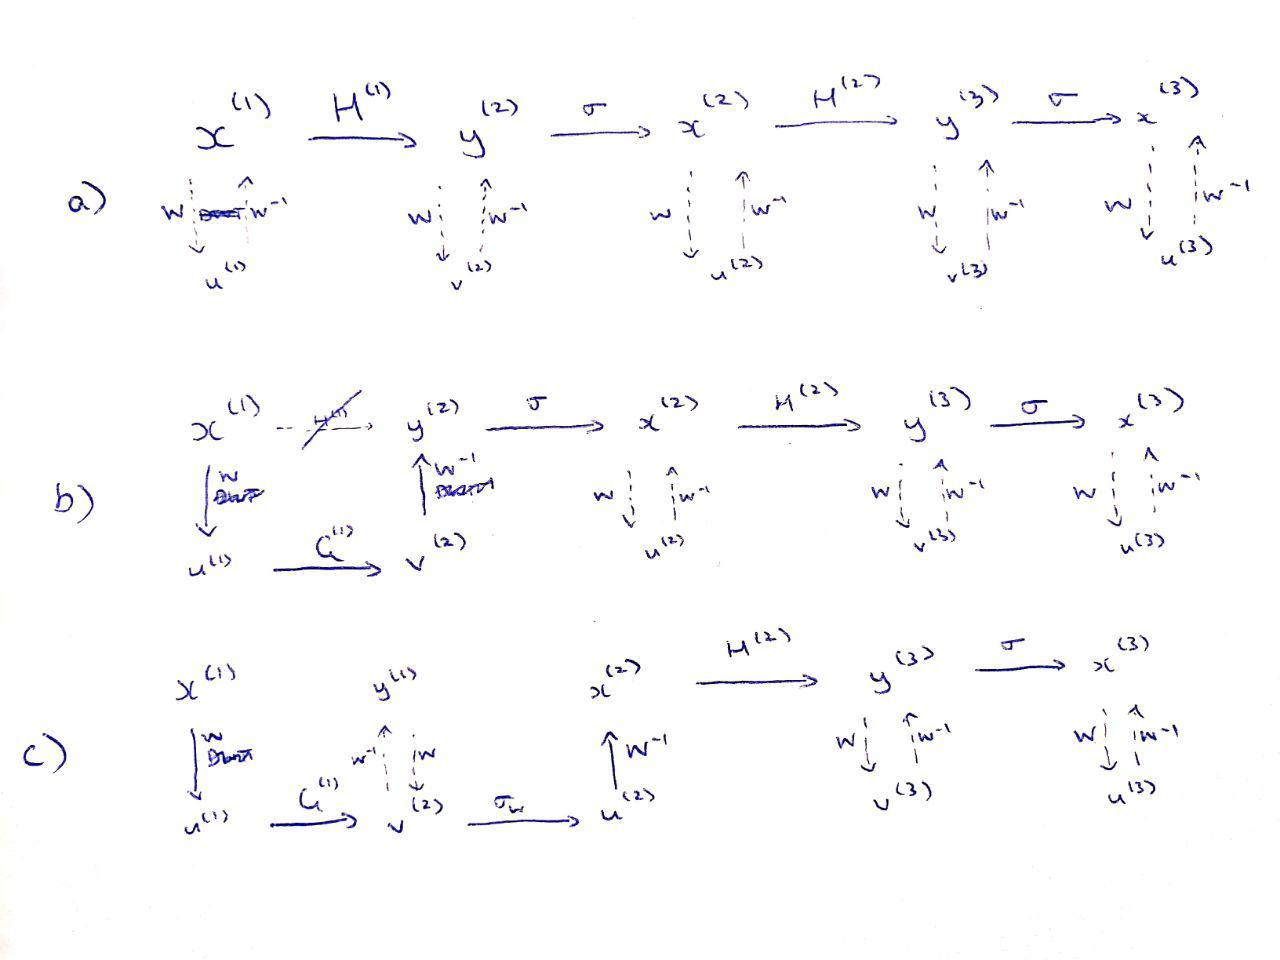
\includegraphics[width=0.8\textwidth]{\imgpath/fwd_chain.jpg}
  \mycaption{Proposed new forward pass in the wavelet domain}{Two network 
  layers with some possible options for processing. Solid lines denote the
  evaluation path and dashed lines indicate relationships. In (a) we see a
  regular convolutional neural network. We have included the dashed lines to
  make clear what we are denoting as $u$ and $v$ with respect to their
  equivalents $x$ and $y$. In (b) we get to $y^{(2)}$ through a different path.
  First we take the wavelet transform of $x^{(1)}$ to give $u^{(1)}$, apply a
  wavelet gain layer $\mathcal{G}^{(1)}$, and take the inverse wavelet transform
  to give $y^{(2)}$. The cross through $\mathcal{H}^{(1)}$ indicates that this
  path is no longer present. Note that there may not be any possible
  $\mathcal{G}^{(1)}$ to make $y^{(2)}$ from (b) equal $y^{(2)}$ from (a). In
  (c) we have stayed in the wavelet domain longer, and applied a wavelet
  nonlinearity $\sigma_w$ to give $u^{(2)}$. We then return to the pixel domain
  to give $x^{(2)}$ and continue on from there in the pixel domain.}
  \label{fig:ch6:fwd_chain}
\end{figure}
At the beginning of each stage of a neural network we have the activations
$x^{(l)}$. Naturally, all of these activations have their equivalent wavelet
coefficients $u^{(l)}$. 

From \eqref{eq:ch6:conv}, convolutional layers also have intermediate
activations $y^{(l)}$. Let us differentiate these from the $x$ coefficients and
modify \eqref{eq:ch6:dwt_coeffs} and \eqref{eq:ch6:dtcwt_coeffs} to say the 
$\DTCWT$ of $y^{(l)}$ gives $v$.

We now propose the wavelet gain layer $G$.
The name `gain layer' comes from the inspiration for this chapter's work, in
that the first layer of CNN could be nearly done in the wavelet domain by
setting subband gains to 0 and 1. 

The gain layer $G$ can be used instead of a convolutional layer. 
It is designed to work on the wavelet coefficients of an activation,
$u$ to give outputs $v$. 

This can be seen as breaking the convolutional path in
\autoref{fig:ch6:fwd_chain} and taking a new route to get to the next layer's
coefficients. From here, we can return to the pixel domain by taking the
corresponding inverse wavelet transform $W^{-1}$. Alternatively, we
can stay in the wavelet domain and apply a wavelet based nonlinearity $\sigma_w$
to give the next layer's $u$ coefficients. Ultimately we would like to explore
architecture design with arbitrary sections in the wavelet and pixel domain, but
to do this we must first explore: 
\begin{itemize}
  \item How effective $G$ is at replacing $H$.
  \item How effective $\sigma_w$ is at replcaing $\sigma$.
\end{itemize}

\subsection{The $\DTCWT$ Gain Layer}
To do the mixing across the $C_l$ channels at each subband, giving $C_{l+1}$
output channels, we introduce the learnable filters:
%
\begin{align}
  g_{lp} &\in \reals[C_{l+1}\x C_l\x k_{lp}\x k_{lp}] \label{eq:ch6:glp} \\
  g_{1,1} &\in \complexes[C_{l+1}\x C_l\x k_1\x k_1] \\
  g_{1,2} &\in \complexes[C_{l+1}\x C_l\x k_1\x k_1] \\
      & \vdots \nonumber \\
  g_{J,6} &\in \complexes[C_{l+1}\x C_l\x k_J\x k_J]  \label{eq:ch6:gj6}
\end{align}
%
where $k$ is the size of the mixing kernels. These could be $1\x 1$ for
simple gain control, or could be larger, say $3\x 3$, to do more complex
filtering on the subbands. 

With these gains we define $v = Gu$ to be:
\begin{align}
  v_{lp}[f, \nn] &=  \sum_{c=0}^{C_l-1} u_{lp}[c, \nn] \conv g_{lp}[f, c, \nn] \\
  v_{1,1}[f, \nn] &=  \sum_{c=0}^{C_l-1} u_{1,1}[c, \nn] \conv g_{1,1}[f, c, \nn] \\
  v_{1,2}[f, \nn] &=  \sum_{c=0}^{C_l-1} u_{1,2}[c, \nn] \conv g_{1,2}[f, c, \nn] \\
                  & \vdots \nonumber \\
  v_{J,6}[f, \nn] &=  \sum_{c=0}^{C_l-1} u_{J,6}[c, \nn] \conv g_{J,6}[f, c, \nn] 
\end{align}

Note that for complex signals $a, b$ the convolution $a \conv b$ is defined as $(a_r \conv
b_r - a_i \conv b_i) + j(a_r \conv b_i + a_i \conv b_r)$. This is shown 
in Figure~\autoref{fig:ch6:dtcwt_blk_diagram}.

\subsubsection{The Output}
Due to the shift invariant properties of the $\DTCWT$, the gain layer can achieve aliasing
cancelling and therefore has a transfer function. The proof of this is done in
\autoref{app:ch6:dtcwt}. 

\begin{figure}[ht!]
  \centering
  \begin{tikzpicture}
    \matrix (m1) [row sep=5mm, column sep=6mm,align=center,anchor=center]
	{
	%--------------------------------------------------------------------
		\node[coordinate]                  (m00) {};    &
		\node[coordinate]                  (m01) {};          &
		\node[dspsquare]                   (m02) {$A_r(z)$};          &
		\node[circle,draw,inner sep=1pt]   (m03) {\downsamplertext{M}}; &
		\node[dspnodeopen,dsp/label=above] (m04) {$U_r(z)$};          &
    \node[rectangle,draw,inner sep=2pt](m05) {$G_{r}(z)$}; &
		\node[dspnodeopen,dsp/label=above] (m06) {$V_r(z)$};          &
		\node[circle,draw,inner sep=1pt]   (m07) {\upsamplertext{M}}; &
		\node[dspsquare]                   (m08) {$S_r(z)$};          &
		\node[coordinate]                  (m09) {};          &
		\node[coordinate]                  (m0X) {};          \\
		%--------------------------------------------------------------------
		\node[]                            (m10) {$X(z)$};          &
		\node[coordinate]                  (m11) {};          &
		\node[coordinate]                  (m12) {};    &
		\node[coordinate]                  (m13) {};          &
		\node[coordinate]                  (m14) {};    &
		\node[coordinate]                  (m15) {};          &
		\node[coordinate]                  (m16) {};    &
		\node[coordinate]                  (m17) {};          &
		\node[coordinate]                  (m18) {};    &
		\node[dspadder]                    (m19) {};          &
    \node[]                            (m1X) {$Y(z)$};          \\
		%--------------------------------------------------------------------
		\node[coordinate]                  (m20) {};    &
		\node[coordinate]                  (m21) {};          &
		\node[dspsquare]                   (m22) {$A_i(z)$};          &
		\node[circle,draw,inner sep=1pt]   (m23) {\downsamplertext{M}}; &
		\node[dspnodeopen,dsp/label=below] (m24) {$U_i(z)$};          &
      \node[rectangle,draw,inner sep=2pt](m25) {$G_{r}(z)$}; &
		\node[dspnodeopen,dsp/label=below] (m26) {$V_i(z)$};          &
		\node[circle,draw,inner sep=1pt]   (m27) {\upsamplertext{M}}; &
		\node[dspsquare]                   (m28) {$S_i(z)$};          &
		\node[coordinate]                  (m29) {};          &
		\node[coordinate]                  (m2X) {};          \\
		%--------------------------------------------------------------------
  };
	\draw[dspline] (m10) -- (m11);
	\draw[dspline] (m11) -- (m01);
	\draw[dspline] (m11) -- (m21);
	\foreach \i in {0,2} {
    	\draw[dspconn] (m\i1) -- (m\i2);
    	\draw[dspconn] (m\i2) -- (m\i3);
    	\draw[dspline] (m\i3) -- (m\i4);
    	\draw[dspconn] (m\i4) -- (m\i5);
    	\draw[dspline] (m\i5) -- (m\i6);
    	\draw[dspconn] (m\i6) -- (m\i7);
    	\draw[dspconn] (m\i7) -- (m\i8);
    	\draw[dspline] (m\i8) -- (m\i9);
	}
	%\draw[dspflow] (m04) --  (m06);
	%\draw[dspflow] (m24) -- (m26);
  \draw[dspconn] (m24) -- node[draw,pos=0.7,inner sep=2pt,fill=white] {$-G_{i}(z)$} (m06);
  \draw[dspconn] (m04) -- node[draw,pos=0.7,inner sep=2pt,fill=white] {$G_{i}(z)$} (m26);
  \draw[dspconn] (m09) -- (m19);
  \draw[dspconn] (m29) -- (m19);
	\draw[dspconn] (m19) -- (m1X);
	
\end{tikzpicture}


  \mycaption{Block Diagram of a single channel 1-D $\DTCWT$ Gain Layer}{Here we show the real and
  imaginary trees for a single subband. Note that while it may look similar to 
  a DWT block diagram, this diagram represents the two trees for one subband rather
  than a single tree with a pair of subbands. The gain layer does a complex
  multiply, using both the real and imaginary parts of the decomposed signal.
  This preserves the shift invariance of the $\DTCWT$ for the reconstructed
  signal $Y$.
  }
  \label{fig:ch6:dtcwt_gain}
\end{figure}

For a single subband in the $\DTCWT$, the gain layer uses a complex learned
weight $g$. \autoref{fig:ch6:dtcwt_gain} shows a single subband $\DTCWT$
based gain layer. 
Let us call the low analysis filters $A = A_r + jA_i$ and 
the synthesis filters $S = S_r + jS_i$ (these are normally called $H$ and
$G$, but we keep those letters reserved for the CNN and gain layer filters). 
The output of this layer is:
\begin{equation}\label{eq:ch6:dtcwt_fwd}
  Y(z) = \frac{2}{M}X(z) \left[G_r(z^{M}) \left(A_r(z)S_r(z) + A_i(z)S_i(z)\right)
  + G_i(z^{M}) \left(A_r(z)S_i(z) - A_i(z)S_r(z)\right) \right] \\
\end{equation}
See \autoref{app:ch6:dtcwt} for the derivation. The $G_r$ term modifies the
subband gain $A_rS_r + A_iS_i$ and the $G_i$ term modifies its Hilbert Pair
$A_rS_i - A_iS_r$. \autoref{fig:ch6:dtcwt_bands} show the contour plots for the
frequency support of each of these subbands. The complex gain $g$ can be used to
reshape the frequency response for each subband independently.

\subsubsection{Backpropagation}\label{sec:ch6:dtcwt_update}
If H were complex, the first term in \autoref{eq:ch6:backprop} would be
$\bar{H}(1/\bar{z})$, but as each individual block in the $\DTCWT$ is purely
real, we can use the simpler form $H(z^{-1})$. 

Again, let us calculate $\Delta V_r(z)$ and $\Delta V_i(z)$ by backpropagating
$\Delta Y(z)$ through the inverse $\DTCWT$. Again this is the same as doing the
forward $\DTCWT$ on $\Delta Y(z)$. Then the weight update equations are:
\begin{align}
  \Delta G_r(z) &= \Delta V_r(z) U_r(z^{-1}) + \Delta V_i(z) U_i(z^{-1})  \label{eq:ch6:gr_update}\\
  \Delta G_i(z) &=  -\Delta V_r(z) U_i(z^{-1}) + \Delta V_i(z) U_r(z^{-1})  \label{eq:ch6:gi_update} 
\end{align}
%
The passthrough equations have similar form to \eqref{eq:ch6:dtcwt_fwd}:
\begin{equation}\label{eq:ch6:dtcwt_passthrough}
    \Delta X(z) = \frac{2\Delta Y(z)}{M} \left[G_r(z^{-M})\left( A_r(z)S_r(z) + A_i(z)S_i(z) \right)\right. + 
      \left. jG_i(z^{-M}) \left(A_r(z)S_i(z) - A_i(z)S_r(z) \right) \right] 
\end{equation}

\begin{figure}[t]
  \centering
  \subfloat[]{%
    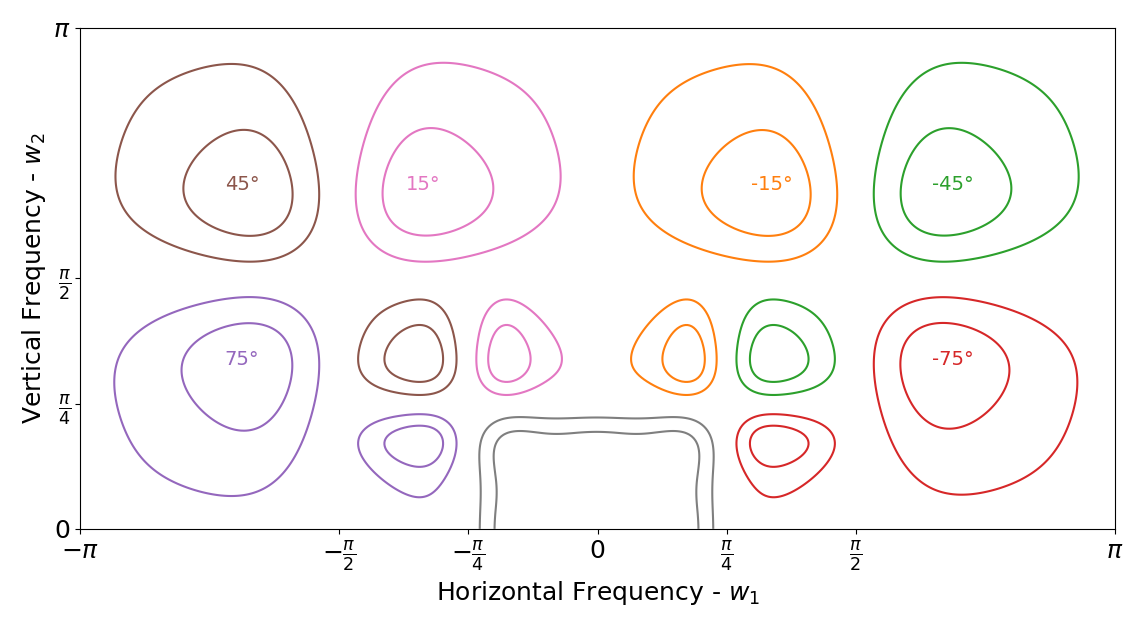
\includegraphics[height=6cm]{\imgpath/subbands.png}
    \label{fig:ch6:dtcwt_bands_freq}
  }
  \hspace{1cm}
%    \newline
  \subfloat[]{%
    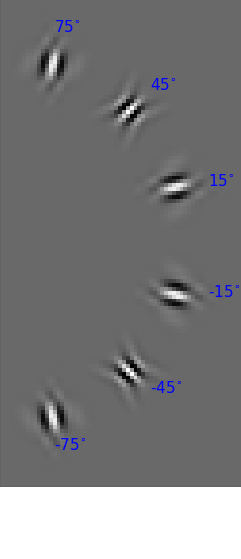
\includegraphics[height=5.7cm]{\imgpath/impulses.png}
    \label{fig:ch6:dtcwt_bands_impulse}
  }
  \mycaption{$\DTCWT$ subbands}{\subref{fig:ch6:dtcwt_bands_freq} -1dB and -3dB contour plots showing
  the support in the Fourier domain of the 6 subbands of the $\DTCWT$ at scales
  1 and 2, and the scale 2 lowpass. These are the product of the single side
  band filters $P(z)$ and $Q(z)$ from \autoref{thm:ch6:shiftinv}.
  \subref{fig:ch6:dtcwt_bands_impulse} The pixel domain impulse responses for
  the second scale wavelets. The Hilbert pair for each wavelet is the underlying
  sinusoid phase shifted by 90 degrees.}
  \label{fig:ch6:dtcwt_bands}
\end{figure}

\begin{figure}[t!]
  \centering
  % \subfloat[]{%
    % \resizebox{\textwidth}{!} {\begin{tikzpicture}[%
  path image/.style={%
    path picture={%
      \node at (path picture bounding box.center) {%
        \includegraphics[height=2.0cm]{#1}
      };
    }
  }, 
  path pic/.style={%
    path picture={%
      \node at (path picture bounding box.center) {%
        \includegraphics[height=0.8cm]{#1}
      };
    }
  }, 
  scale=0.6]

  \draw (8.8, 2.5, 5) node {\Large{$\mathtt{u}^{(l)}$}};
  \draw (10.0, 2.3, 5) node {\Large{$\conv$}};
  \draw (11.5, 2.45, 5) node {\Large{$\mathtt{g}^{(l)}$}};
  \draw (15, 2.5, 5) node {\Large{$\mathtt{v}^{(l+1)}$}};
  \draw (18.5, 2.5, 5) node {\Large{$\mathtt{u}^{(l+1)}$}};
  \draw (25, 0.8, 3.5) node {\Large{$x^{(l+1)}$}};
  \draw[<->] (10, -1.3, 2) -- (10, 0.5, 2) node[near end, right] {$C_{l+1}$};

  \draw [decorate,decoration={brace,mirror,amplitude=10pt,raise=4pt},yshift=0pt]
    (3.8,-2.5,-4) -- (4.8,-2.5,15) node [black,midway,xshift=0.8cm];
  \draw [->, fill=gray!30,ultra thick] (0.5, -2.5, 4) -- (2.5, -2.5, 4)
    node[midway, above] {$\F{DWT}$};

  \draw [decorate,decoration={brace,amplitude=10pt,raise=4pt},yshift=0pt]
    (16.5,-2.5,-4) -- (18,-2.5,15) node [black,midway,xshift=0.8cm];
  \draw [->, fill=gray!30,ultra thick] (19, -2.5, 4) -- (21.5, -2.5, 4)
    node[midway, above] {$\F{DWT}^{-1}$};
  \tikzcuboid{
  shiftx=-2.5cm,
  shifty=-2.5cm,
  shiftz=7,
  scale=0.5,
  anglex=0, 
  angley=90, 
  anglez=230,
  dimx=3, 
  dimy=3, 
  dimz=6,
  densityx=1, 
  densityy=1, 
  densityz=1,
  shade=false,
  emphedge=true,
  shadeopacity=0,
  emphstyle/.style={rounded corners=0.2pt,line width=0.3mm},
  front/.style={draw=blue!50!white,fill=blue!50!white},%
  right/.style={draw=blue!50!white,fill=blue!50!white},%
  top/.style={draw=blue!50!white,fill=blue!50!white},%
  drawxdims=true,
  dimxval=W,
  drawydims=true,
  dimyval=H,
  drawzdims=true,
  dimzval=C_l,
  }

  % Draw the 6 subband activations and their filters
  \foreach \i in {1,...,2} {
    \tikzcuboid{
    shiftx=6cm,
    shifty=-2.0cm,
    shiftz=-5+5*\i,
    scale=0.5,
    dimx=2, dimy=2, dimz=3,
    densityx=4, densityy=4, densityz=2,
    drawxdims=false,
    drawydims=false,
    dimzval=C_l,
    drawzdims=false,
    front/.style={draw=blue!50!white,fill=blue!50!white},%
    right/.style={draw=blue!50!white,fill=blue!50!white},%
    top/.style={draw=blue!50!white,fill=blue!50!white},%
    }
    \tikzcuboid{
    dimz=2,
    shiftx=12.0cm,
    }
    \tikzcuboid{
    shiftx=16.0cm,
    }
    \draw [->, fill=gray!30,ultra thick] (10+0.1*\i, -1.5, -2+2.5*\i) -- (11+0.1*\i, -1.5, -2+2.5*\i);
      % node[midway, above] {$\sigma_w$};
    \draw [->, fill=gray!30,ultra thick] (14+0.1*\i, -1.5, -2+2.5*\i) -- (15+0.1*\i, -1.5, -2+2.5*\i)
      node[midway, above] {$\sigma_w$};

    \tikzcuboid{
    shiftx=8.5cm,
    shifty=-1.0cm,
    shiftz=-5+5*\i,
    dimx=0.4, dimy=0.4, dimz=3,
    densityx=5, densityy=5, densityz=2,
    front/.style={draw=red!50!white,fill=red!50!white},%
    right/.style={draw=red!50!white,fill=red!50!white},%
    top/.style={draw=red!50!white,fill=red!50!white},%
    }
    \tikzcuboid{
    shifty=-1.5cm,
    }
    \tikzcuboid{
    shifty=-2.0cm,
    }
    \tikzcuboid{
    shifty=-2.5cm,
    }
    % \draw (8cm, -1.8cm, -15+5*\i) node {$\vdots$};
  }
  \tikzcuboid{
  shiftx=6cm,
  shifty=-2.0cm,
  shiftz=10,
  scale=0.5,
  dimx=2, dimy=2, dimz=3,
  densityx=4, densityy=4, densityz=2,
  dimxval=\frac{W}{2},
  drawxdims=true,
  dimyval=\frac{H}{2},
  drawydims=true,
  dimzval=C_l,
  drawzdims=true,
  front/.style={draw=blue!50!white,fill=blue!50!white},%
  right/.style={draw=blue!50!white,fill=blue!50!white},%
  top/.style={draw=blue!50!white,fill=blue!50!white},%
  }
  \tikzcuboid{
  shiftx=12.0cm,
  dimz=2,
  dimzval=C_{l+1},
  }
  \tikzcuboid{
  shiftx=16.0cm,
  drawxdims=false,
  drawydims=false,
  drawzdims=false
  }
  \draw [->, fill=gray!30,ultra thick] (10+3*0.1, -1.5, 5.5) -- (11+3*0.1, -1.5, 5.5);
    % node[midway, above] {$\sigma_w$};
  \draw [->, fill=gray!30,ultra thick] (14+3*0.1, -1.5, 5.5) -- (15+3*0.1, -1.5, 5.5)
      node[midway, above] {$\sigma_w$};
  \tikzcuboid{
  shiftx=8.5cm,
  shifty=-1.0cm,
  shiftz=10,
  dimx=0.4, dimy=0.4, dimz=3,
  drawxdims=false,
  drawydims=false,
  drawzdims=false,
  densityx=5, densityy=5, densityz=2,
  front/.style={draw=red!50!white,fill=red!50!white},%
  right/.style={draw=red!50!white,fill=red!50!white},%
  top/.style={draw=red!50!white,fill=red!50!white},%
  }
  \tikzcuboid{
  shifty=-1.5cm,
  }
  \tikzcuboid{
  shifty=-2.0cm,
  }
  \tikzcuboid{
  shifty=-2.5cm,
  }

  % Draw the lowpass activation and its set of filters
  \tikzcuboid{
  shiftx=6cm,
  shifty=-2.0cm,
  shiftz=30,
  scale=0.5,
  dimx=3, dimy=3, dimz=4,
  densityx=4, densityy=4, densityz=2,
  dimxval=W,
  drawxdims=true,
  dimyval=H,
  drawydims=true,
  dimzval=C_l,
  drawzdims=true,
  front/.style={draw=blue!50!white,fill=blue!50!white},%
  right/.style={draw=blue!50!white,fill=blue!50!white},%
  top/.style={draw=blue!50!white,fill=blue!50!white},%
  }
  \tikzcuboid{
  shiftx=12.0cm,
  dimz=3,
  drawxdims=false,
  drawydims=false,
  dimzval=C_{l+1},
  drawzdims=true
  }
  \tikzcuboid{
  shiftx=16.0cm,
  drawzdims=false,
  }
  \draw [->, fill=gray!30,ultra thick] (11, -1.5, 14.5) -- (12, -1.5, 14.5);
    % node[midway, above] {$\sigma_w$};
  \draw [->, fill=gray!30,ultra thick] (15, -1.5, 14.5) -- (16, -1.5, 14.5)
    node[midway, above] {$\sigma_w$};

  \tikzcuboid{
  shiftx=9cm,
  shifty=-2.75cm,
  dimx=0.8, dimy=0.8, dimz=3,
  drawxdims=false,
  drawydims=false,
  drawzdims=false,
  densityx=5, densityy=5, densityz=2,
  front/.style={draw=red!50!white,fill=red!50!white},%
  right/.style={draw=red!50!white,fill=red!50!white},%
  top/.style={draw=red!50!white,fill=red!50!white},%
  }
  \tikzcuboid{
  shifty=-2.00cm,
  }
  \tikzcuboid{
  shifty=-1.25cm,
  }
  \tikzcuboid{
  shifty=-0.5cm,
  }
  \tikzcuboid{
  shiftx=23cm,
  shifty=-2.5cm,
  shiftz=7,
  scale=0.5,
  anglex=0, 
  angley=90, 
  anglez=230,
  dimx=3, 
  dimy=3, 
  dimz=6,
  densityx=1, 
  densityy=1, 
  densityz=1,
  shade=false,
  emphedge=true,
  shadeopacity=0,
  emphstyle/.style={rounded corners=0.2pt,line width=0.3mm},
  front/.style={draw=blue!50!white,fill=blue!50!white},%
  right/.style={draw=blue!50!white,fill=blue!50!white},%
  top/.style={draw=blue!50!white,fill=blue!50!white},%
  drawxdims=true,
  dimxval=W,
  drawydims=true,
  dimyval=H,
  drawzdims=true,
  dimzval=C_{l+1},
  }
  % \draw (0, .3, 0) node {\large{$x^{(l)}$}};

\end{tikzpicture}
}
    % \label{fig:ch6:dwt_blk_diagram}
  % }\newline
  % \vspace{1cm}
  % \subfloat[]{%
    % \resizebox{\textwidth}{!} {\begin{tikzpicture}[%
  path image/.style={%
    path picture={%
      \node at (path picture bounding box.center) {%
        \includegraphics[height=2.0cm]{#1}
      };
    }
  }, 
  path pic/.style={%
    path picture={%
      \node at (path picture bounding box.center) {%
        \includegraphics[height=0.8cm]{#1}
      };
    }
  }, 
  scale=0.6]
  \draw (-1, 0.8, 3.5) node {\Large{$x^{(l)}$}};
  \draw (8.5, 2.5, 0) node {\Large{$u^{(l)}$}};
  \draw (9.7, 2.3, 0) node {\Large{$\conv$}};
  \draw (11, 2.5, 0) node {\Large{$g^{(l)}$}};
  \draw (15, 2.5, 0) node {\Large{$v^{(l+1)}$}};
  \draw (18.5, 2.5, 0) node {\Large{$u^{(l+1)}$}};
  \draw (25, 0.8, 3.5) node {\Large{$x^{(l+1)}$}};
  \draw[<->] (10, -1, -2) -- (10, 0.9, -2) node[near end, right] {$C_{l+1}$};

  \draw (1.0, -2.5, -3) node {bandpass};
  \draw (2.0, -2.5, 14) node {lowpass};
  \draw [decorate,decoration={brace,mirror,amplitude=10pt,raise=4pt},yshift=0pt]
    (3.8,-2.5,-8) -- (4.8,-2.5,18) node [black,midway,xshift=0.8cm];
  \draw [->, fill=gray!30,ultra thick] (0.5, -2.5, 4) -- (2.5, -2.5, 4)
    node[midway, above] {$\DTCWT$};
  \tikzcuboid{
  shiftx=-2.5cm,
  shifty=-2.5cm,
  shiftz=7,
  scale=0.5,
  anglex=0, 
  angley=90, 
  anglez=230,
  dimx=3, 
  dimy=3, 
  dimz=6,
  densityx=1, 
  densityy=1, 
  densityz=1,
  shade=false,
  emphedge=true,
  shadeopacity=0,
  emphstyle/.style={rounded corners=0.2pt,line width=0.3mm},
  front/.style={draw=blue!50!white,fill=blue!50!white},%
  right/.style={draw=blue!50!white,fill=blue!50!white},%
  top/.style={draw=blue!50!white,fill=blue!50!white},%
  drawxdims=true,
  dimxval=W,
  drawydims=true,
  dimyval=H,
  drawzdims=true,
  dimzval=C_l,
  }

  % Draw the 6 subband activations and their filters
  \foreach \i in {1,...,5} {
    \tikzcuboid{
    shiftx=6cm,
    shifty=-2.0cm,
    shiftz=-15+5*\i,
    scale=0.5,
    dimx=2, dimy=2, dimz=3,
    densityx=4, densityy=4, densityz=2,
    drawxdims=false,
    drawydims=false,
    dimzval=C_l,
    drawzdims=false,
    front/.style={draw=blue!90!white,fill=blue!90!white},%
    right/.style={draw=blue!90!white,fill=blue!90!white},%
    top/.style={draw=blue!90!white,fill=blue!90!white},%
    }
    \tikzcuboid{
    dimz=2,
    shiftx=12.0cm,
    }
    \tikzcuboid{
    shiftx=16.0cm,
    }
    \draw [->, fill=gray!30,ultra thick] (9.8+0.08*\i, -1.5, -7+2.5*\i) -- (10.8+0.08*\i, -1.5, -7+2.5*\i);
      % node[midway, above] {$\sigma_w$};
    \draw [->, fill=gray!30,ultra thick] (13.8+0.08*\i, -1.5, -7+2.5*\i) -- (14.8+0.08*\i, -1.5, -7+2.5*\i)
      node[midway, above] {$\sigma_w$};

    \tikzcuboid{
    shiftx=8.5cm,
    shifty=-1.0cm,
    shiftz=-15+5*\i,
    dimx=0.4, dimy=0.4, dimz=3,
    densityx=5, densityy=5, densityz=2,
    front/.style={draw=red!90!white,fill=red!90!white},%
    right/.style={draw=red!90!white,fill=red!90!white},%
    top/.style={draw=red!90!white,fill=red!90!white},%
    }
    \tikzcuboid{
    shifty=-1.5cm,
    }
    \tikzcuboid{
    shifty=-2.0cm,
    }
    \tikzcuboid{
    shifty=-2.5cm,
    }
    % \draw (8cm, -1.8cm, -15+5*\i) node {$\vdots$};
  }
  \tikzcuboid{
  shiftx=6cm,
  shifty=-2.0cm,
  shiftz=15,
  scale=0.5,
  dimx=2, dimy=2, dimz=3,
  densityx=4, densityy=4, densityz=2,
  dimxval=\frac{W}{2},
  drawxdims=true,
  dimyval=\frac{H}{2},
  drawydims=true,
  dimzval=C_l,
  drawzdims=true,
  front/.style={draw=blue!90!white,fill=blue!90!white},%
  right/.style={draw=blue!90!white,fill=blue!90!white},%
  top/.style={draw=blue!90!white,fill=blue!90!white},%
  }
  \tikzcuboid{
  shiftx=12.0cm,
  dimz=2,
  dimzval=C_{l+1},
  }
  \tikzcuboid{
  shiftx=16.0cm,
  drawxdims=false,
  drawydims=false,
  drawzdims=false
  }
  \draw [->, fill=gray!30,ultra thick] (9.8+6*0.08, -1.5, 8) -- (10.8+6*0.08, -1.5, 8);
    % node[midway, above] {$\sigma_w$};
  \draw [->, fill=gray!30,ultra thick] (13.8+6*0.08, -1.5, 8) -- (14.8+6*0.08, -1.5, 8)
      node[midway, above] {$\sigma_w$};
  \tikzcuboid{
  shiftx=8.5cm,
  shifty=-1.0cm,
  shiftz=15,
  dimx=0.4, dimy=0.4, dimz=3,
  drawxdims=false,
  drawydims=false,
  drawzdims=false,
  densityx=5, densityy=5, densityz=2,
  front/.style={draw=red!90!white,fill=red!90!white},%
  right/.style={draw=red!90!white,fill=red!90!white},%
  top/.style={draw=red!90!white,fill=red!90!white},%
  }
  \tikzcuboid{
  shifty=-1.5cm,
  }
  \tikzcuboid{
  shifty=-2.0cm,
  }
  \tikzcuboid{
  shifty=-2.5cm,
  }

  % Draw the lowpass activation and its set of filters
  \tikzcuboid{
  shiftx=6cm,
  shifty=-2.0cm,
  shiftz=35,
  scale=0.5,
  dimx=3, dimy=3, dimz=4,
  densityx=4, densityy=4, densityz=2,
  dimxval=W,
  drawxdims=true,
  dimyval=H,
  drawydims=true,
  dimzval=C_l,
  drawzdims=true,
  front/.style={draw=blue!50!white,fill=blue!50!white},%
  right/.style={draw=blue!50!white,fill=blue!50!white},%
  top/.style={draw=blue!50!white,fill=blue!50!white},%
  }
  \tikzcuboid{
  shiftx=12.0cm,
  dimz=2,
  drawxdims=true,
  drawydims=true,
  dimzval=C_{l+1},
  drawzdims=true
  }
  \tikzcuboid{
  shiftx=16.0cm,
  drawxdims=false,
  drawydims=false,
  drawzdims=false,
  }
  \draw [->, fill=gray!30,ultra thick] (11.2, -1.5, 17.5) -- (12.0, -1.5, 17.5);
    % node[midway, above] {$\sigma_w$};
  \draw [->, fill=gray!30,ultra thick] (15.5, -1.5, 17.5) -- (16.5, -1.5, 17.5)
    node[midway, above] {$\sigma_w$};

  \tikzcuboid{
  shiftx=9cm,
  shifty=-2.75cm,
  dimx=0.8, dimy=0.8, dimz=3,
  drawxdims=false,
  drawydims=false,
  drawzdims=false,
  densityx=5, densityy=5, densityz=2,
  front/.style={draw=red!50!white,fill=red!50!white},%
  right/.style={draw=red!50!white,fill=red!50!white},%
  top/.style={draw=red!50!white,fill=red!50!white},%
  }
  \tikzcuboid{
  shifty=-2.00cm,
  }
  \tikzcuboid{
  shifty=-1.25cm,
  }
  \tikzcuboid{
  shifty=-0.5cm,
  }
  \tikzcuboid{
  shiftx=23cm,
  shifty=-2.5cm,
  shiftz=7,
  scale=0.5,
  anglex=0, 
  angley=90, 
  anglez=230,
  dimx=3, 
  dimy=3, 
  dimz=6,
  densityx=1, 
  densityy=1, 
  densityz=1,
  shade=false,
  emphedge=true,
  shadeopacity=0,
  emphstyle/.style={rounded corners=0.2pt,line width=0.3mm},
  front/.style={draw=blue!50!white,fill=blue!50!white},%
  right/.style={draw=blue!50!white,fill=blue!50!white},%
  top/.style={draw=blue!50!white,fill=blue!50!white},%
  drawxdims=true,
  dimxval=W,
  drawydims=true,
  dimyval=H,
  drawzdims=true,
  dimzval=C_{l+1},
  }
  % \draw (0, .3, 0) node {\large{$x^{(l)}$}};
  \draw [decorate,decoration={brace,amplitude=10pt,raise=4pt},yshift=0pt]
    (16.5,-2.5,-8) -- (18,-2.5,18) node [black,midway,xshift=0.8cm];
  \draw [->, fill=gray!30,ultra thick] (19, -2.5, 4) -- (21.5, -2.5, 4)
    node[midway, above] {$\DTCWT^{-1}$};

\end{tikzpicture}
}
  \resizebox{\textwidth}{!}{\begin{tikzpicture}[%
  path image/.style={%
    path picture={%
      \node at (path picture bounding box.center) {%
        \includegraphics[height=2.0cm]{#1}
      };
    }
  }, 
  path pic/.style={%
    path picture={%
      \node at (path picture bounding box.center) {%
        \includegraphics[height=0.8cm]{#1}
      };
    }
  }, 
  scale=0.6]
  \draw (-1, 0.8, 3.5) node {\Large{$x^{(l)}$}};
  \draw (8.5, 2.5, 0) node {\Large{$u^{(l)}$}};
  \draw (9.7, 2.3, 0) node {\Large{$\conv$}};
  \draw (11, 2.5, 0) node {\Large{$g^{(l)}$}};
  \draw (15, 2.5, 0) node {\Large{$v^{(l+1)}$}};
  \draw (18.5, 2.5, 0) node {\Large{$u^{(l+1)}$}};
  \draw (25, 0.8, 3.5) node {\Large{$x^{(l+1)}$}};
  \draw[<->] (10, -1, -2) -- (10, 0.9, -2) node[near end, right] {$C_{l+1}$};

  \draw (1.0, -2.5, -3) node {bandpass};
  \draw (2.0, -2.5, 14) node {lowpass};
  \draw [decorate,decoration={brace,mirror,amplitude=10pt,raise=4pt},yshift=0pt]
    (3.8,-2.5,-8) -- (4.8,-2.5,18) node [black,midway,xshift=0.8cm];
  \draw [->, fill=gray!30,ultra thick] (0.5, -2.5, 4) -- (2.5, -2.5, 4)
    node[midway, above] {$\DTCWT$};
  \tikzcuboid{
  shiftx=-2.5cm,
  shifty=-2.5cm,
  shiftz=7,
  scale=0.5,
  anglex=0, 
  angley=90, 
  anglez=230,
  dimx=3, 
  dimy=3, 
  dimz=6,
  densityx=1, 
  densityy=1, 
  densityz=1,
  shade=false,
  emphedge=true,
  shadeopacity=0,
  emphstyle/.style={rounded corners=0.2pt,line width=0.3mm},
  front/.style={draw=blue!50!white,fill=blue!50!white},%
  right/.style={draw=blue!50!white,fill=blue!50!white},%
  top/.style={draw=blue!50!white,fill=blue!50!white},%
  drawxdims=true,
  dimxval=W,
  drawydims=true,
  dimyval=H,
  drawzdims=true,
  dimzval=C_l,
  }

  % Draw the 6 subband activations and their filters
  \foreach \i in {1,...,5} {
    \tikzcuboid{
    shiftx=6cm,
    shifty=-2.0cm,
    shiftz=-15+5*\i,
    scale=0.5,
    dimx=2, dimy=2, dimz=3,
    densityx=4, densityy=4, densityz=2,
    drawxdims=false,
    drawydims=false,
    dimzval=C_l,
    drawzdims=false,
    front/.style={draw=blue!90!white,fill=blue!90!white},%
    right/.style={draw=blue!90!white,fill=blue!90!white},%
    top/.style={draw=blue!90!white,fill=blue!90!white},%
    }
    \tikzcuboid{
    dimz=2,
    shiftx=12.0cm,
    }
    \tikzcuboid{
    shiftx=16.0cm,
    }
    \draw [->, fill=gray!30,ultra thick] (9.8+0.08*\i, -1.5, -7+2.5*\i) -- (10.8+0.08*\i, -1.5, -7+2.5*\i);
      % node[midway, above] {$\sigma_w$};
    \draw [->, fill=gray!30,ultra thick] (13.8+0.08*\i, -1.5, -7+2.5*\i) -- (14.8+0.08*\i, -1.5, -7+2.5*\i)
      node[midway, above] {$\sigma_w$};

    \tikzcuboid{
    shiftx=8.5cm,
    shifty=-1.0cm,
    shiftz=-15+5*\i,
    dimx=0.4, dimy=0.4, dimz=3,
    densityx=5, densityy=5, densityz=2,
    front/.style={draw=red!90!white,fill=red!90!white},%
    right/.style={draw=red!90!white,fill=red!90!white},%
    top/.style={draw=red!90!white,fill=red!90!white},%
    }
    \tikzcuboid{
    shifty=-1.5cm,
    }
    \tikzcuboid{
    shifty=-2.0cm,
    }
    \tikzcuboid{
    shifty=-2.5cm,
    }
    % \draw (8cm, -1.8cm, -15+5*\i) node {$\vdots$};
  }
  \tikzcuboid{
  shiftx=6cm,
  shifty=-2.0cm,
  shiftz=15,
  scale=0.5,
  dimx=2, dimy=2, dimz=3,
  densityx=4, densityy=4, densityz=2,
  dimxval=\frac{W}{2},
  drawxdims=true,
  dimyval=\frac{H}{2},
  drawydims=true,
  dimzval=C_l,
  drawzdims=true,
  front/.style={draw=blue!90!white,fill=blue!90!white},%
  right/.style={draw=blue!90!white,fill=blue!90!white},%
  top/.style={draw=blue!90!white,fill=blue!90!white},%
  }
  \tikzcuboid{
  shiftx=12.0cm,
  dimz=2,
  dimzval=C_{l+1},
  }
  \tikzcuboid{
  shiftx=16.0cm,
  drawxdims=false,
  drawydims=false,
  drawzdims=false
  }
  \draw [->, fill=gray!30,ultra thick] (9.8+6*0.08, -1.5, 8) -- (10.8+6*0.08, -1.5, 8);
    % node[midway, above] {$\sigma_w$};
  \draw [->, fill=gray!30,ultra thick] (13.8+6*0.08, -1.5, 8) -- (14.8+6*0.08, -1.5, 8)
      node[midway, above] {$\sigma_w$};
  \tikzcuboid{
  shiftx=8.5cm,
  shifty=-1.0cm,
  shiftz=15,
  dimx=0.4, dimy=0.4, dimz=3,
  drawxdims=false,
  drawydims=false,
  drawzdims=false,
  densityx=5, densityy=5, densityz=2,
  front/.style={draw=red!90!white,fill=red!90!white},%
  right/.style={draw=red!90!white,fill=red!90!white},%
  top/.style={draw=red!90!white,fill=red!90!white},%
  }
  \tikzcuboid{
  shifty=-1.5cm,
  }
  \tikzcuboid{
  shifty=-2.0cm,
  }
  \tikzcuboid{
  shifty=-2.5cm,
  }

  % Draw the lowpass activation and its set of filters
  \tikzcuboid{
  shiftx=6cm,
  shifty=-2.0cm,
  shiftz=35,
  scale=0.5,
  dimx=3, dimy=3, dimz=4,
  densityx=4, densityy=4, densityz=2,
  dimxval=W,
  drawxdims=true,
  dimyval=H,
  drawydims=true,
  dimzval=C_l,
  drawzdims=true,
  front/.style={draw=blue!50!white,fill=blue!50!white},%
  right/.style={draw=blue!50!white,fill=blue!50!white},%
  top/.style={draw=blue!50!white,fill=blue!50!white},%
  }
  \tikzcuboid{
  shiftx=12.0cm,
  dimz=2,
  drawxdims=true,
  drawydims=true,
  dimzval=C_{l+1},
  drawzdims=true
  }
  \tikzcuboid{
  shiftx=16.0cm,
  drawxdims=false,
  drawydims=false,
  drawzdims=false,
  }
  \draw [->, fill=gray!30,ultra thick] (11.2, -1.5, 17.5) -- (12.0, -1.5, 17.5);
    % node[midway, above] {$\sigma_w$};
  \draw [->, fill=gray!30,ultra thick] (15.5, -1.5, 17.5) -- (16.5, -1.5, 17.5)
    node[midway, above] {$\sigma_w$};

  \tikzcuboid{
  shiftx=9cm,
  shifty=-2.75cm,
  dimx=0.8, dimy=0.8, dimz=3,
  drawxdims=false,
  drawydims=false,
  drawzdims=false,
  densityx=5, densityy=5, densityz=2,
  front/.style={draw=red!50!white,fill=red!50!white},%
  right/.style={draw=red!50!white,fill=red!50!white},%
  top/.style={draw=red!50!white,fill=red!50!white},%
  }
  \tikzcuboid{
  shifty=-2.00cm,
  }
  \tikzcuboid{
  shifty=-1.25cm,
  }
  \tikzcuboid{
  shifty=-0.5cm,
  }
  \tikzcuboid{
  shiftx=23cm,
  shifty=-2.5cm,
  shiftz=7,
  scale=0.5,
  anglex=0, 
  angley=90, 
  anglez=230,
  dimx=3, 
  dimy=3, 
  dimz=6,
  densityx=1, 
  densityy=1, 
  densityz=1,
  shade=false,
  emphedge=true,
  shadeopacity=0,
  emphstyle/.style={rounded corners=0.2pt,line width=0.3mm},
  front/.style={draw=blue!50!white,fill=blue!50!white},%
  right/.style={draw=blue!50!white,fill=blue!50!white},%
  top/.style={draw=blue!50!white,fill=blue!50!white},%
  drawxdims=true,
  dimxval=W,
  drawydims=true,
  dimyval=H,
  drawzdims=true,
  dimzval=C_{l+1},
  }
  % \draw (0, .3, 0) node {\large{$x^{(l)}$}};
  \draw [decorate,decoration={brace,amplitude=10pt,raise=4pt},yshift=0pt]
    (16.5,-2.5,-8) -- (18,-2.5,18) node [black,midway,xshift=0.8cm];
  \draw [->, fill=gray!30,ultra thick] (19, -2.5, 4) -- (21.5, -2.5, 4)
    node[midway, above] {$\DTCWT^{-1}$};

\end{tikzpicture}
}
  \label{fig:ch6:dtcwt_blk_diagram}
  \mycaption{Block diagram of proposed method to learn in the wavelet domain}{
  Activations are shaded blue and learned parameters red. The input $x^{(l)}\in
  \mathbb{R}^{C_l\x H\x W}$ is taken into the wavelet domain and each subband is
  mixed independently with $C_{l+1}$ sets of convolutional filters (this is what
  we call the \emph{wavelet gain layer}. After mixing, a possible wavelet nonlinearity 
  $\sigma_w$ is applied to the subbands, before returning to the pixel domain
  with an inverse wavelet transform.}
  \label{fig:ch6:block_diagrams}
\end{figure}

\subsection{Examples}
\autoref{fig:ch6:examples} show example impulse responses of the $\DTCWT$ gain
layer. For comparison, we also show similar `impulse responses' for a gain layer
done in the DWT domain \footnote{modifying DWT coefficients causes a loss of the
alias cancellation properties so these are not true impulse response}. The DWT 
outputs come from three random variables: a $1\x 1$ 
convolutional weight applied to each of the low-high, high-low and high-high
subbands. The $\DTCWT$ outputs come from twelve random variables. Again a $1\x
1$ convolutional weight, but now applied to six complex subbands. 
Our experiments have shown that the distribution of the normalized
cross-correlation between 512 of such randomly generated shapes for the DWT matches the
distribution for random vectors with roughly 2.8 degrees of freedom (c.f. 3
random variables in the layer). Similarly for the $\DTCWT$, the distribution of
the normalized cross-correlation matches the distribution for random vectors
with roughtly 11.5 degrees of freedom (c.f. 12 random variables in the layer).
This is particularly reassuring for the $\DTCWT$ as it is showing that there is
still representatitve power despite the redundancy of the transform.

\begin{figure}
  \centering
  \subfloat[]{%
    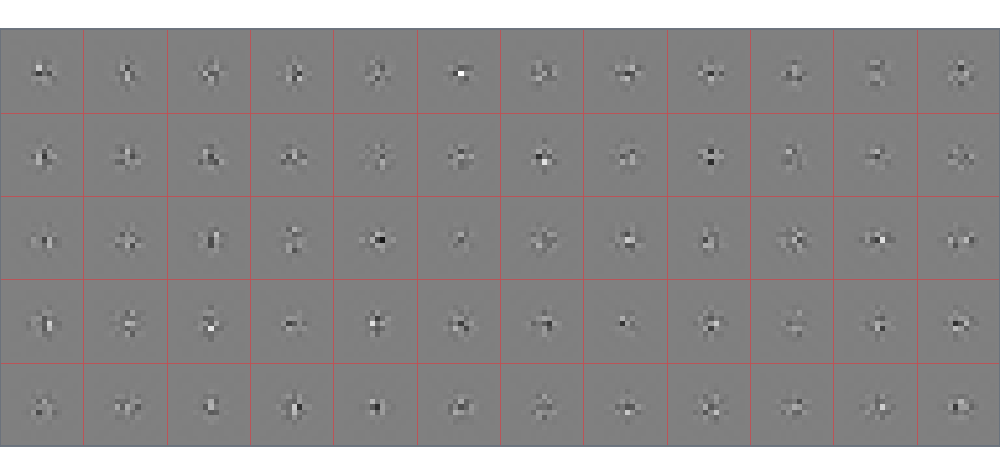
\includegraphics[width=\textwidth]{\imgpath/dtcwt_examples.png}
    \label{fig:ch6:dtcwt_examples}
  }
  \newline
  \subfloat[]{%
  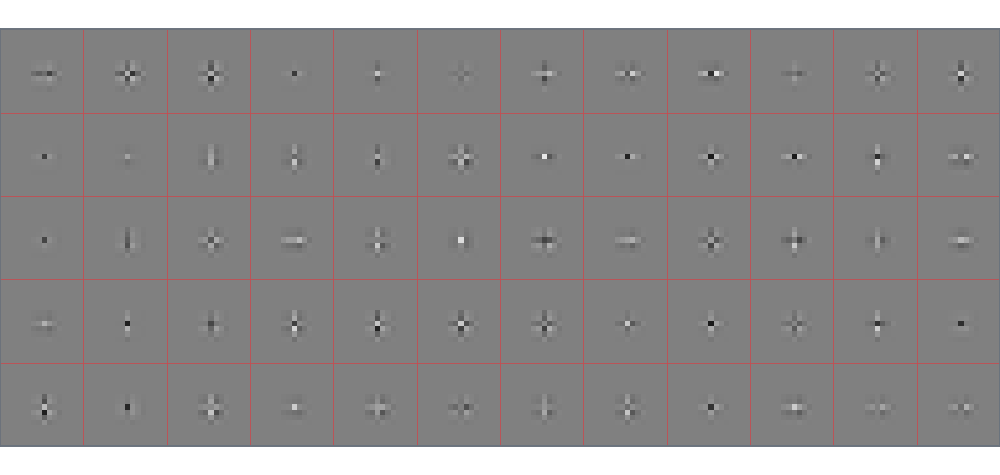
\includegraphics[width=\textwidth]{\imgpath/dwt_examples.png}
    \label{fig:ch6:dwt_examples}
  }
  \mycaption{Example outputs from an impulse input for the proposed gain layers}{
  Example outputs $y = W^{-1}GWx$ for an impulse
  $x$ for the $\DTCWT$ gain layer and for a similarly designed DWT gain layer.
  \subref{fig:ch6:dtcwt_examples} shows the output $y$ for a $\DTCWT$ based
  system. $g_{lp} = 0$ and $g_1$ has spatial size $1\x 1$. The 12 values
  in $g_1$ are independently sampled from a random normal of variance 1.
  The 60 samples come from 60 different random draws of the weights.
  \subref{fig:ch6:dwt_examples}
  shows the outputs $y$ when $x$ is an impulse and $W$ is the DWT with a
  `db2' wavelet family. The strong horizontal and vertical properties of the DWT
  can clearly be seen in comparison to the much freer $\DTCWT$.}
  \label{fig:ch6:examples}
\end{figure}


\subsection{Implementation Details}
Before analyzing its performance, we compare the implementation properties of
our proposed layer to a standard convolutional layer.

\subsubsection{Parameter Memory Cost}\label{sec:ch6:memory}
A standard convolutional layer with $C_l$ input channels, $C_{l+1}$ output channels
and kernel size $L\x L$ has $L^2C_{l}C_{l+1}$ parameters, with $L=3$ or $L=5$
common choices for the spatial size.
\begin{equation}
  \text{\#conv params} = 9C_lC_{l+1}
\end{equation}

We must choose the spatial sizes of both the lowpass and bandpass
mixing kernels. In our work, we set the spatial support of the lowpass 
filters for the $\DTCWT$ gain layer to be $1\x 1$ and the support of the 
complex bandpass filters to be $1\x 1$.
%
Further, we typically limit ourselves initially to only considering a single scale
transform. If we wish, we can decompose the input into more scales, resulting in a larger
net area of effect. In particular, it may be useful to do a two scale transform and discard 
the first scale coefficients. This does not increase the number of gains to
learn, but changes the position of the bands in the frequency space.

This means the number of parameters is:
\begin{equation}
  \text{\#params} = (2\x 6 + 1)C_lC_{l+1} = 13C_lC_{l+1} \label{eq:ch6:memcost2}
\end{equation} 
%
This is slightly larger than the $9C_lC_{l+1}$ parameters used in a
standard $3\x 3$ convolution, but as \autoref{fig:ch6:examples} shows, the
spatial support of the full filter is larger than an equivalent one
parameterized in the filter domain. 

\subsubsection{Activation Memory Cost}\label{sec:ch6:act_memory}
A standard convolutional layer needs to save the activation $x^{(l)}$ to
convolve with the backpropagated gradient $\dydx{L}{y^{(l+1)}}$ on the backwards
pass (to give $\dydx{L}{w^{(l)}}$). For an input with $C_l$ channels of spatial
size $H\x W$, this means
%
\begin{equation}
  \text{\#conv floats} = HWC_l 
\end{equation}

Our layers require us to save the wavelet coefficients $u_{lp}$ and  $u_{j,k}$
for updating the $g$ terms as in \eqref{eq:ch6:g_update} and
\eqref{eq:ch6:gr_update}, \eqref{eq:ch6:gi_update}.  For the critically sampled
DWT, this requires:
%
\begin{equation}
  \text{\#DWT floats} = HWC_l 
\end{equation}
%
to be saved for the backwards pass. For the $4:1$ redundant $\DTCWT$, this 
requires:
%
\begin{equation}
  \text{\#$\DTCWT$ floats} = 4HWC_l 
\end{equation}
%
to be saved for the backwards pass.  You can see this difference from the
difference in the block diagrams in \autoref{fig:ch6:block_diagrams}.

Note that a single scale $\DTCWT$ gain layer requires $16/7$ times as many
floats to be saved as compared to the invariant layer of the previous chapter.
The extra cost of this comes from two things. Firstly, we keep the real and
imaginary components for the bandpass (as opposed to only the magnitude),
meaning we need $3HWC_l$ floats, rather than $\frac{3}{2}HWC_l$. Additionally,
the lowpass was downsampled in the previous chapter, requiring only
$\frac{1}{4}HWC_l$, whereas we keep the full sample rate costing $HWC_l$.

If memory is an issue and the computation of the $\DTCWT$ is very fast, then we
only need to save the $x^(l)$ coefficients and can calculate the $u$'s on the
fly during the backwards pass. Note that a two scale $\DTCWT$ gain layer would
still only require $4HWC_l$ floats.

\subsubsection{Computational Cost}\label{sec:ch6:computation}
A standard convolutional layer with kernel size $L\x L$ needs $L^2C_{l+1}$
multiplies per input pixel (of which there are $C_{l}\x H\x W$).

For the DWT with Daubechies 2 filters, the forward and inverse transform only
require about $6$ multiplies per input pixel. The mixing is then done at a
reduced spatial resolution. For our proposed kernel sizes of $3\x 3$ for the
lowpass and $1\x 1$ for the bandpass, the DWT gain layer requires:

\begin{equation}
  % \frac{7}{4}C_{l+1} + 48 \label{eq:comp}
  \text{\#DWT mults/pixel} = \underbrace{\hphantom{1} \frac{3}{4}C_{l+1} \hphantom{1}}_{\textrm{bandpass}} +
  \underbrace{\hphantom{1}\vphantom{\frac{3}{4}} \frac{3^2}{4} C_{l+1} \hphantom{1}}_{\textrm{lowpass}} + 
  \underbrace{\vphantom{\frac{3}{4}} 6}_{\text{DWT}} + 
  \underbrace{\vphantom{\frac{3}{4}} 6}_{\text{DWT}^{-1}} = \quad 4C_{l+1} + 12 \quad
  \label{eq:ch6:comp_dwt}
\end{equation}

This is smaller than a standard $3\x 3$ convolutional layer using $9C_{l+1}$
multiplies per pixel.

For the $\DTCWT$, the overhead calculations are the same as in
\autoref{sec:ch5:computation}, so we will omit their derivation here. The mixing
is however different, requiring complex convolution for the bandpass
coefficients, and convolution over a higher resolution lowpass. The bandpass has
one quarter spatial resolution at the first scale, but this is offset by the
$4:1$ cost of complex multiplies compared to real multiplies. Again assuming we
have set $J=1$ and $k_{lp} = 3$ then the total cost for the gain layer is:
%
\begin{equation}
  % \frac{7}{4}C_{l+1} + 48 \label{eq:comp}
  \text{\#$\DTCWT$ mults/pixel} = \underbrace{\hphantom{1} \frac{6\x 4}{4}C_{l+1} \hphantom{1}}_{\textrm{bandpass}} +
  \underbrace{\hphantom{1}\vphantom{\frac{6}{4}} C_{l+1} \hphantom{1}}_{\textrm{lowpass}} + 
  \underbrace{\vphantom{\frac{6}{4}} 36}_{\DTCWT} + 
  \underbrace{\vphantom{\frac{6}{4}} 36}_{\DTCWT^{-1}} = \quad 7C_{l+1} + 72 \quad
  \label{eq:ch6:comp_dtcwt}
\end{equation}
This is marginally smaller than a $3\x 3$ convolutional layer.

\subsubsection{Parameter Initialization}
For both layer types we use the Glorot Initialization scheme \cite{glorot_understanding_2010}
with $a=1$: 
%
\begin{equation}
  g_{ij} \drawnfrom U\left[ -\sqrt{\frac{6}{(C_l + C_{l+1})k^2}},\ \sqrt{\frac{6}{(C_l + C_{l+1})k^2}}\
  \right] \label{eq:ch6:glorot}
\end{equation}
where $k$ is the kernel size.
% \subsection{Forward and Backward Algorithm}
% Algorithm~\autoref{alg:ch6:inv}.
% \begin{algorithm}[tb]
\caption{Locally Invariant Convolutional Layer forward and backward
passes}\label{alg:ch6:inv}
\begin{algorithmic}[1]
\Procedure{GAINLAYERFWD}{$x,\ g_{lp},\ g_1$}
\State $u_{lp},\ u_{1} \gets \DTCWT(x^l, \mbox{nlevels}=1) $ \Comment{$u_{1}$ has 6 orientations and is complex}
  \State \textbf{save} $u_{lp},\ u_{1}$ \Comment{For the backwards pass}
  \State $v_{lp} \gets u_{lp} \conv g_{lp}$ 
  \For{$1\leq k \leq 6$}
  \State \begin{varwidth}[t]{\linewidth}  $v_{1,k} \gets 
      \left( \real{u_{1,k}} \conv \real{g_{1,k}} - \imag{u_{1,k}} \conv \imag{g_{1,k}} \right)\ +$ \par
      \hskip\algorithmicindent \hphantom{abc}$ j\left(\real{u_{1,k}} \conv \imag{g_{1,k}} + \imag{u_{1,k}} \conv \real{g_{1,k}}\right)$;
  \end{varwidth}
  \EndFor
  \State $y \gets \DTCWT^{-1}(v_{lp}, v_{1})$
  \State \textbf{return} $y$
\EndProcedure
\end{algorithmic}\vspace{10pt}
\begin{algorithmic}[1]
  \Procedure{GAINLAYERBWD}{$\dydx{L}{Y},\ g_{lp},\ g_1$}
  \State \textbf{load} $u_{lp},\ u_1$
  \State \textbf{return} $\dydx{L}{x},\ \dydx{L}{A}$
\EndProcedure
\end{algorithmic}
\end{algorithm}


